\section{Introduction}\label{sec:zero-shot-intro}


Attributes are high-level descriptions of visual concepts. In contrast to categories, which broadly classify objects or scenes based on high-level features, attributes often remain continuous or a variable that can change across instances of the same category. For instance, in the "outdoor scene" category, attributes can be associated with seasonal transitions (e.g., winter to spring), weather changes (e.g., rainy, sunny), or time of day (e.g., daylight, sunset, night).  In this work, I focus on such transient attributes that dynamically shape the visual appearance of an outdoor scene.

\begin{figure}[ht]
  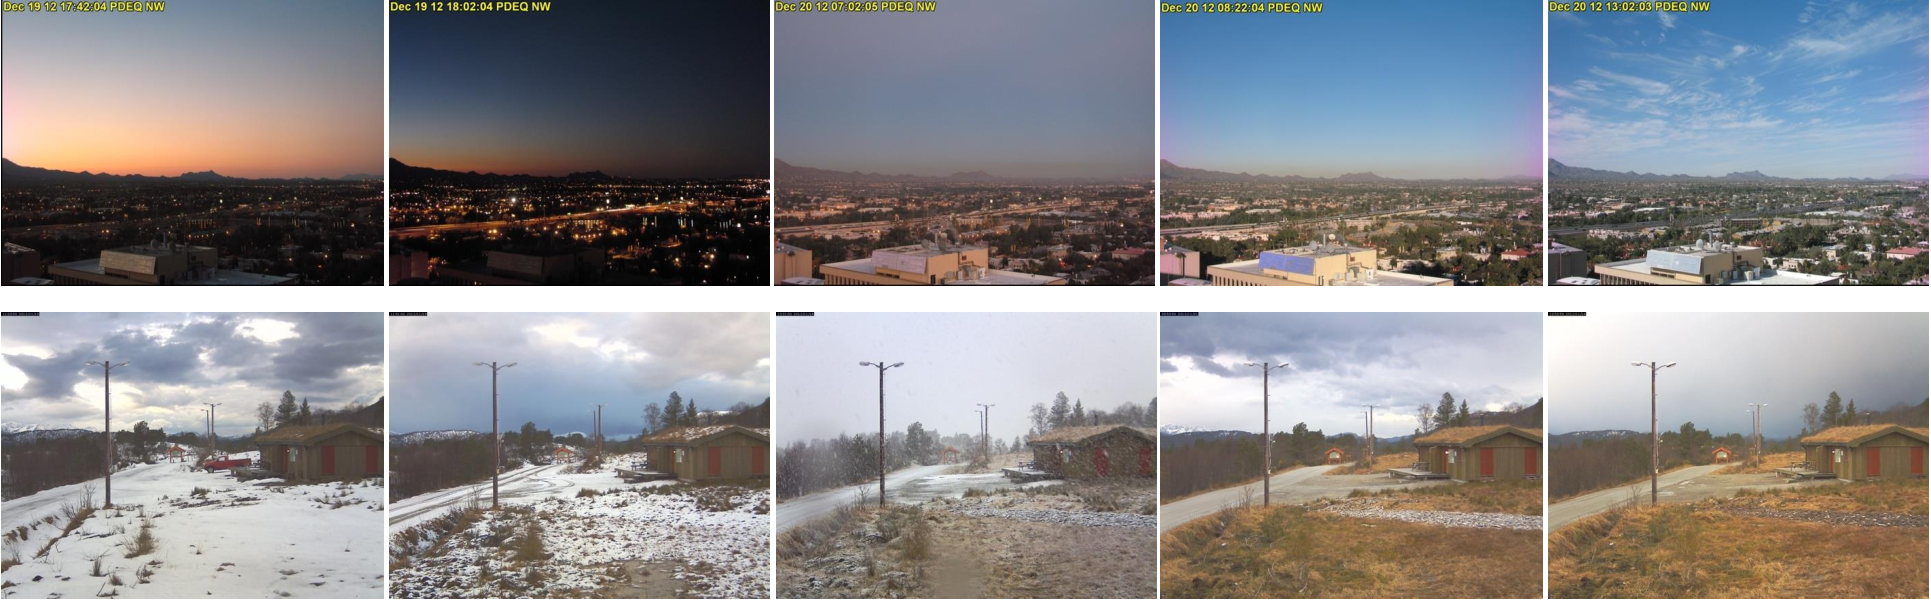
\includegraphics[width=\textwidth]{Chapters/zero-shot-tat-figs/tat-teaser.pdf}
  \caption{Transition of the illumination throughout the day or the weather changes across seasons alter the scene appearance significantly in terms of colour, tone, texture, and style. However, main content, such as the structure, permanent objects, etc. remains unchanged. Transient attribute transfer aims to capture alterations related to such temporal effects. Images from the Transient Attribute Dataset \cite{laffont2014transient}.}
  \label{fig:zero-shot-teaser}
\end{figure}

Transient attributes influence our perception of a scene by altering appearance related properties, such as colour, texture, and overall atmosphere, i.e., style and tone. From the slow transition of sunrise to daylight, the accumulation of snow on the ground, to the clearing sky after an overcast day, these attributes define the dynamic and captivating nature of the visual world. Recent works in the computer vision/graphics fields have engaged with the transfer of such attributes either under the umbrella term of high-level image editing or standalone. Capturing such temporal changes plays a crucial role in a range of applications, such as photography, filmmaking, gaming, and virtual and augmented reality for producing photorealistic simulation. However, the accurate transfer of transient attributes is highly challenging due to the requirement of a deep understanding of the scene components as well as maintaining essential content. 


This chapter aims to address these challenges by exploring recent advancements in generative models, more specifically diffusion-based approaches. The observation that fine-tuning these foundation models with a small dataset can lead to overfitting motivates me to leverage the pre-trained models to guide the transfer process in a way that improves the generalisability. Therefore, I focus on a zero-shot approach that eliminates the need for extensive additional datasets, instead utilising the robust priors embedded in foundation models. I evaluate this approach through qualitative comparisons with fine-tuned models and demonstrate its ability to effectively capture the transfers, such as seasonal changes and varying lighting and weather conditions while preserving the scene's core features.

%By advancing the understanding and manipulation of transient scene attributes, this research contributes to the broader goal of enhancing the realism and flexibility of visual content generation, paving the way for more immersive and contextually adaptive visual experiences.

In summary, this chapter contributes to the broader goal of manipulating appearance in a data-efficient manner by: 

%Multiple Transformation Blending
\begin{itemize}

   \item exploiting a pre-trained diffusion model in a zero-shot setting and requiring only an input image and a text prompt, a single word, describing the target attribute,
    
   \item capturing the ever-changing transitions in an outdoor scene without any explicit decomposition of scene components.

\end{itemize}
